This task focused on predicting Vietnamese gold prices using a linear regression model implemented in PySpark.
The objective was to transform historical time-series data into a suitable format for regression,
train a model, and evaluate its predictive performance.

\subsection{Overview of Linear Regression}
\label{subsec:overview-of-linear-regression}

Linear Regression is a supervised learning algorithm that models the linear relationship between a continuous target variable ($y$) and one or more independent predictor variables (features $\mathbf{x}$). The goal is to find an optimal linear function that best predicts $y$ given $\mathbf{x}$.

For a single feature $x$, the model is:
\begin{equation}
    y = \beta_0 + \beta_1 x + \epsilon
    \label{eq:simple_lr}
\end{equation}
With multiple features $x_1, x_2, \ldots, x_p$, it extends to:
\begin{equation}
    y = \beta_0 + \beta_1 x_1 + \beta_2 x_2 + \ldots + \beta_p x_p + \epsilon
    \label{eq:multiple_lr}
\end{equation}
where $\beta_0$ is the intercept, $\beta_j$ are the feature coefficients (weights), and $\epsilon$ is the error term. The coefficients are typically learned by minimizing a loss function, such as Mean SquaredError (MSE), often using optimization algorithms like L-BFGS. Key assumptions include linearity, independence of errors, and homoscedasticity. This project applies linear regression to predict gold prices based on historical price features.

\subsection{Data Preparation}
\label{subsec:data-preparation}
\begin{itemize}
    \item \textbf{Dataset:} The primary data source was \texttt{gold\_prices.csv} (2009/08/01 to 2025/01/01),
    read into a PySpark DataFrame.
    \item \textbf{Feature Engineering:} For each target date $t$, features were the respective `Buy Price' or `Sell Price' values from the 10 consecutive preceding days.
    PySpark's \texttt{Window} functions and \texttt{lag} operation were used, followed by \texttt{VectorAssembler} to create feature vectors (e.g., \texttt{Previous Buy Price(s)}). 4000 samples were generated (\texttt{random\_state=38}).
    \item \textbf{Data Splitting:} The generated DataFrame was randomly split into training (70\%) and testing (30\%) sets (\texttt{seed=2}).
\end{itemize}

\subsection{Model Implementation and Training}
\label{subsec:model-implementation-and-training}

Two separate linear regression models (\texttt{pyspark.ml.regression.LinearRegression}) were developed: one for `Buy Price' and one for `Sell Price', using their respective 10-day historical price vectors as features and the current price as the label.
Models were configured with the \texttt{'l-bfgs'} solver and trained on the 70\% training subset.

\subsection{Experimental Results and Evaluation}
\label{subsec:experimental-results-and-evaluation}

The performance of the trained models was evaluated on both training and testing sets.
Key metrics are summarized in Table~\ref{tab:task2_metrics}.
The R² values (consistently $>$ 0.999), low RMSE/MAE, and high Explained Variance scores indicate strong predictive accuracy and good generalization to unseen data, with no significant overfitting observed.

\begin{table}[h]
    \centering
    \caption{LR Performance Metrics for Gold Price Prediction.}
    \renewcommand{\arraystretch}{1} % Adjust row spacing
    \begin{tabular}{|c|c|c|c|c|c|c|}
        \hline
        \textbf{Model}        & \textbf{Data Set} & \textbf{RMSE} & \textbf{MSE} & \textbf{R²} & \textbf{MAE} & \textbf{Expl. Var.} \\
        \hline
        \multirow{Buy Price}  & Training          & 0.3232        & 0.1045       & 0.9995      & 0.1450       & 225.7249            \\
        \cline{2-7}           & Test              & 0.2975        & 0.0885       & 0.9996      & 0.1356       & 226.5322            \\
        \hline
        \multirow{Sell Price} & Training          & 0.3062        & 0.0938       & 0.9996      & 0.1406       & 240.1171            \\
        \cline{2-7}           & Test              & 0.2913        & 0.0848       & 0.9996      & 0.1319       & 240.6501            \\
        \hline
    \end{tabular}
    \label{tab:task2_metrics}
\end{table}

\subsection{Visualizations}
\label{subsec:visualizations}

\subsubsection{Loss History During Training}\text{}

Line chart (Fig.~\ref{fig:buy_price_model_loss}) illustrated the objective function value per iteration, showing rapid convergence for `Buy Price' model.

\begin{figure}[H]
    \centering
    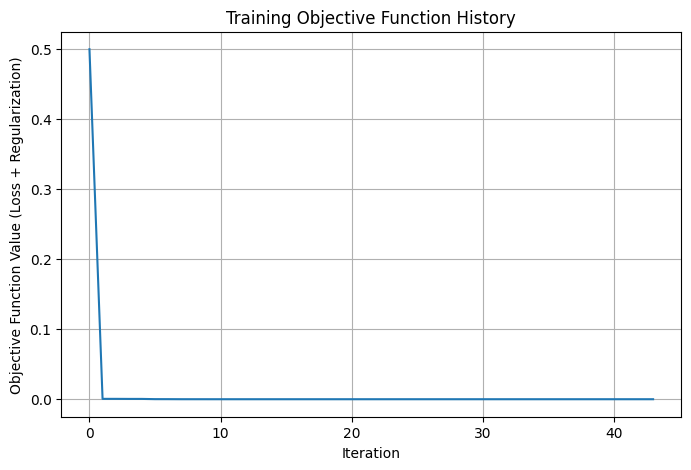
\includegraphics[width=\linewidth]{images/buy_price_model_loss}
    \caption{Loss History of Buy Price Prediction Model}
    \label{fig:buy_price_model_loss}
\end{figure}

\subsubsection{Performance Comparison}\text{}

Bar charts (Fig.~\ref{fig:buy_rmse_mse_r2_mae} nd Fig.~\ref{fig:buy_var}) contrasted evaluation metrics (RMSE, MSE, R$^2$, MAE, Explained Variance) between training and testing sets, visually confirming robust generalization.

\begin{figure}[H]
    \centering
    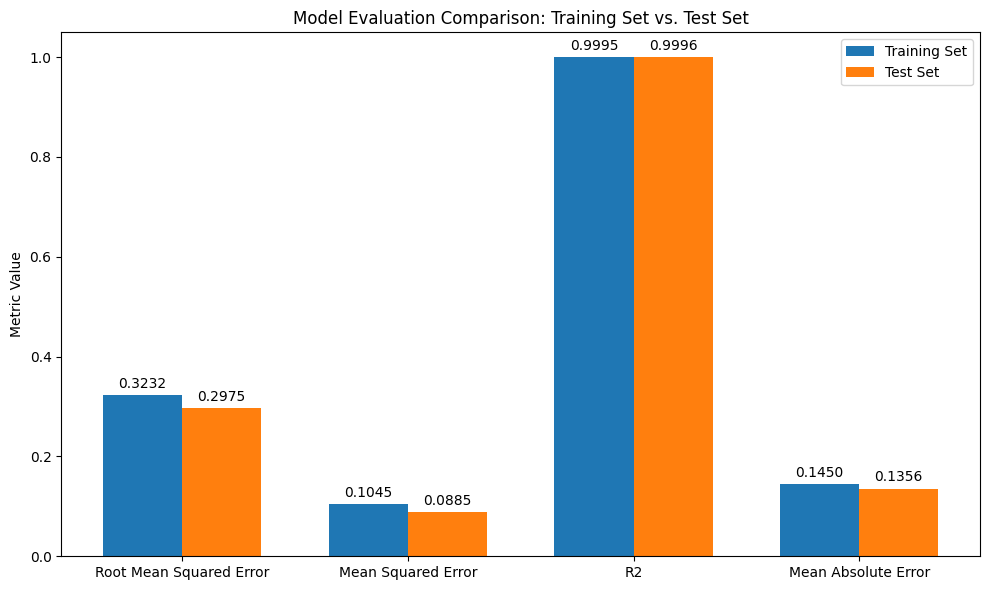
\includegraphics[width=\linewidth]{images/buy_rmse_mse_r2_mae}
    \caption{'Buy Price' Model Performance (Training vs. Test Set).}
    \label{fig:buy_rmse_mse_r2_mae}
\end{figure}

\begin{figure}[H]
    \centering
    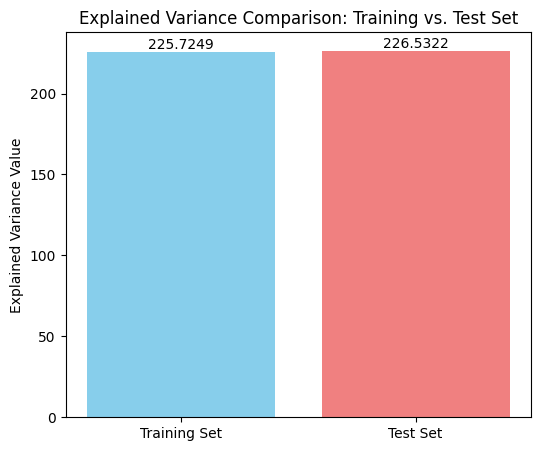
\includegraphics[width=0.8\linewidth]{images/buy_var}
    \caption{'Buy Price' Model Explained Variance Performance (Training vs. Test Set).}
    \label{fig:buy_var}
\end{figure}